\subsubsection{The Model}
\label{subsec:model}

The model used in this application is made up of a series of ellipses to create a two-dimensional side-view figure. Figure~\ref{fig:modelellipses} shows a sketch of this figure:

\begin{figure}[H]
    \centering
	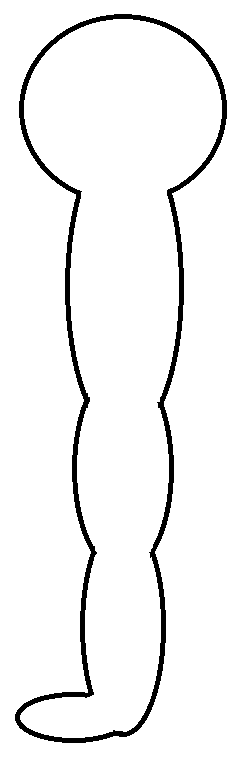
\includegraphics[height=7cm]{algorithm/images/model}
\caption{A sketch of the elliptical model}
\label{fig:modelellipses}
\end{figure}

The model is defined by the following parameters:

\begin{itemize}
	\item \textbf{Scale} A single scale factor to define the size of the model
	\item \textbf{Toe Coordinates} The location of the toes in the frame
	\item \textbf{Angles} Several angles to define the model's pose:
		\begin{enumerate}
			\item Shoulder
			\item Hip
			\item Knee
			\item Ankle
			\item Toe
		\end{enumerate}
\end{itemize}

The angles are each defined from the horizontal plane, and are located at each of the models joints, where the ellipses interlock. These angles are shown in figure~\ref{fig:modelangles}.

\begin{figure}[H]
    \centering
	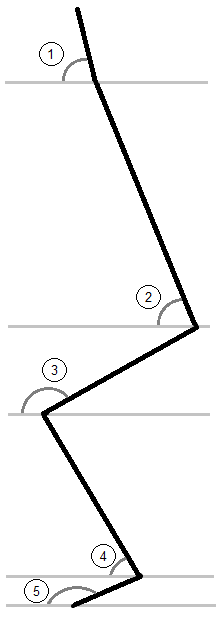
\includegraphics[height=10cm]{algorithm/images/model_angles}
\caption{The five angles defining the model's pose}
\label{fig:modelangles}
\end{figure}

During the tracking phase, the toe coordinates and scale are fixed and the fitting is performed over the five angles in the model. This means that the model has relatively view parameters, which reduces the degrees of freedom and therefore the search-space of the optimisation.

Another advantage of the angles defining the model's position is that it is easy to query the model for information about its current posture. Easy calculations can be made as to whether the model is in the correct position by checking that angles are within an acceptable range.

This two-dimensional model provides enough information to determine that the majority of factors affecting a squat's safety and validity are upheld. A three-dimensional model may have been more accurate and provided more information, but the increased number of degrees of freedom and the additional overhead of rendering a three-dimensional model during fitting would be too large to allow real-time tracking, especially with the limited processing power of a mobile device.

Due to the barbell being a relatively large part of the silhouette, a circle is drawn on the shoulders. This allows for more accurate tracking, keeping the shoulders in line. Figure~\ref{fig:modeldrawn} shows the model when drawn on an empty frame.

\begin{figure}[H]
    \centering
	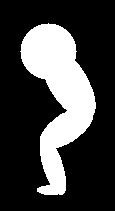
\includegraphics[height=7cm]{algorithm/images/model_drawn}
\caption{The elliptical model drawn on a blank frame}
\label{fig:modeldrawn}
\end{figure}

The model defines the length and width of each of its elliptical components. These are defined as absolute values, but are scaled by the constant scale factor to fit the height of the figure in view. This means that the lifter can be of any height, but a drawback is that should their proportions be different (for example long legs and a short torso), the model will not fit as accurately.

The model also defines minimum and maximum values for each of its angles. These are based on the limitations of the human body, although are reasonably relaxed to allow for maximum freedom. These restrictions reduce the search space in the optimisation, giving a faster and more accurate fit.
